\documentclass[spanish, fleqn]{article}
\usepackage{babel}
\usepackage[utf8]{inputenc}
\usepackage{amsmath}
\usepackage{amsfonts}
\usepackage{wasysym}
\usepackage[colorlinks, urlcolor=blue]{hyperref}
\usepackage[top = 2.5cm, bottom = 2cm, left = 2cm, right = 2cm]{geometry}
\usepackage{listings}
\usepackage{color}
\usepackage{tikz}
\usetikzlibrary{plotmarks}

\definecolor{gris}{rgb}{0.2,0.2,0.2}

%Datos de error
\begin{filecontents}{f1_bis.data}
	# i error
	0 	0.500000007451
	1 	0.749999992549
	2 	0.124999992549
	3 	0.187500007451
	4 	0.0312500074506
	5 	0.0468749925494
	6 	0.00781249254942
	7 	0.0117187574506
	8 	0.00195313245058
	9 	0.00292968004942
	10 	0.000488273799419
\end{filecontents}
\begin{filecontents}{f2_bis.data}
	# i error
	0 	1.49999999441
	1 	0.249999994412
	2 	0.375000005588
	3 	0.0625000055879
	4 	0.0937499944121
	5 	0.0156249944121
	6 	0.0234375055879
	7 	0.00390625558794
	8 	0.00585936941206
	9 	0.000976556912065
	10 	0.00146484933794
\end{filecontents}
\begin{filecontents}{f4_bis.data}
	# i error
	0 	1.49999999534
	1 	0.250000004657
	2 	0.624999995343
	3 	0.187499995343
	4 	0.0312500046566
	5 	0.0781249953434
	6 	0.0234374953434
	7 	0.00390625465661
	8 	0.00976562034339
	9 	0.00292968284339
	10 	0.000488285906613
\end{filecontents}
\begin{filecontents}{f5_bis.data}
	# i error
	0 	1.00000000559
	1 	0.249999994412
	2 	0.375000005588
	3 	0.0625000055879
	4 	0.0937499944121
	5 	0.0156249944121
	6 	0.0234375055879
	7 	0.00390625558794
	8 	0.00585936941206
	9 	0.000976556912065
	10 	0.00146484933794
\end{filecontents}
\begin{filecontents}{f6_bis.data}
	# i error
	0 	0.358407346532
	1 	0.391592653468
	2 	0.0165926534683
	3 	0.170907346532
	4 	0.0771573465317
	5 	0.0302823465317
	6 	0.00684484653175
	7 	0.00487390346825
	8 	0.000985471531749
	9 	0.00194421596825
	10 	0.000479372218251
\end{filecontents}
\begin{filecontents}{f7_bis.data}
	# i error
%	0 	4.57079632487
%	1 	1.07079632487
	2 	0.679203675129
	3 	0.195796324871
	4 	0.241703675129
	5 	0.0229536751285
	6 	0.0864213248715
	7 	0.0317338248715
	8 	0.00439007487148
	9 	0.00928180012852
	10 	0.00244586262852
\end{filecontents}

\begin{filecontents}{f1_newt.data}
	# i error
	0 	0.00633290964665381
	1 	0
\end{filecontents}
\begin{filecontents}{f2_newt.data}
	# i error
	0 	0
\end{filecontents}
\begin{filecontents}{f4_newt.data}
	# i error
	0 	0
\end{filecontents}
\begin{filecontents}{f5_newt.data}
	# i error
	0 	0
\end{filecontents}
\begin{filecontents}{f6_newt.data}
	# i error
	0 	0.652426258902
	1 	0.30427404277
	2 	0.0215405925331
	3 	0.000144408205087
	4 	0.00000000663694432745
	5 	0.0
\end{filecontents}
\begin{filecontents}{f7_newt.data}
	# i error
	0 	0.164254097025
	1 	0.015979453478
	2 	0.000161223676029
	3 	0.0000000165463081014
	4 	0.000000000000000222044604925
	5 	0.0
\end{filecontents}


\title{ILI 285 \\ Laboratorio \#2}
\author{Alonso Sandoval Acevedo\\asandova@alumnos.inf.utfsm.cl\\201073011-5 
		\and Hernán Vargas Leighton\\hvargas@alumnos.inf.utfsm.cl\\201073009-3}
\date{\today}

\begin{document}
\maketitle

\thispagestyle{empty}

\section{Descripción del experimento}
	%Descripción del experimento y suposiciones
	Entre la gran variedad de métodos para obtener las raíces trabajaremos con
	dos muy utilizados como son el método de la bisección y el 	método de 
	Newton. Analizaremos objetivamente los pros y contras de cada	uno de
	ellos comparando algunos de sus aspectos. Por lo visto en clases esperamos
	que el método de bisección tenga una fácil implementación y, a pesar de
	que su tiempo de ejecución debería ser alto, nos entregue buenos
	resultados, por otra parte, el método de Newton debería ser un poco más
	difícil de implementar pero debería ser mucho más rápido.
\section{Desarrollo}
	%Desarrollo y análisis de resultados
	\subsection{Encontrando los ceros}
	\begin{enumerate}
		\item
			Uno de los requisitos para poder utilizar el método de la bisección
			es que la función evaluada en los extremos del rango $[a,b]$ cumpla
			con que $f(a)\cdot f(b)<0$, es decir, un cambio de signo entre $a$ 
			y $b$. Entre las funciones a las que debemos encontrarles raíces
			notamos que algunas de ellas no cumplen con este requisito, por
			ellos fueron modificadas de la siguiente manera:
			\newcommand{\ra}{\rightarrow}
			\begin{gather*}
				f_1 = 	1 - \frac{\sin{x}}{x} = 0 \ra 1 = \frac{\sin{x}}{x} \ra
				x = \sin{x} \ra 0 = \sin{x} - x \ra f_1 = \sin{x} - x \\
				f_2 = x^{10} \ra x^{10} = (x^5)^2 \ra f_2 = x^5\\
				f_4 = | x - 10 | \ra f_4 = x - 10
			\end{gather*}
			Para $f_2$ sabemos que la única raíz de $x^2$ es $0$, por ello, el
			problema puede simplificarse a obtener la raíz de $x^5$. Por otro
			lado, para $f_4$ nos servirá tanto la raíz de $10-x$ como la de 
			$x-10$ pues lo dentro del valor absoluto es lineal.
			Para $f_3$ tenemos el problema de que las raíces son $\pm\infty$\\
			Nuestra implementación de bisección recibe como parámetros una
			función y un intervalo desde \textsf{a} hasta \textsf{b} y
			encuentra una raíz en dicho intervalo.

		\item
			En el método de Newton se utilizó la librería "sympy" para el
			manejo algebraico, obtención de derivadas y límite para casos de
			indefinición (división por cero principalmente). Para las funciones
			de Bessel, se utilizó, tal como en el caso anterior, la librería 
			"scipy", la cual retorna las soluciones de las funciones de Bessel
			y su respectiva derivada para cierto parámetro ($x_0$ en este caso)
			.\\
			Se implementó el método de Newton visto en clases, para cual, antes
			de evaluar cada función se hace un "test" para chequear la posible
			multiplicidad de raíces. Con las 5 primeras iteraciones, se analiza
			el error lineal ($\frac{e_{i+1}}{e_{i}}$), el cual, al ser
			relativamente constante (con respecto a una tolerancia definida),
			se determina la multiplicidad a través de este valor:
			\begin{center}
				$S = \frac{m-1}{m} \rightarrow m = \frac{1}{1-S}$
			\end{center}
			Haciendo un redondeo superior obtenemos un valor aproximado de la
			multiplicidad, en las funciones de la tarea, calzan exactamente.
			Si ($\frac{e_{i+1}}{e_{i}}$) no es constante, se utiliza
			multiplicidad = 1.\\
			Así, en los casos de existir raíz múltiple, se utiliza el método
			de newton mejorado.\\
			Los errores en tiempo de ejecución se calculan entre el valor
			actual y el anterior ($|x_i - x_0|$), al momento de encontrar una
			raíz, se obtienen los errores con respecto a esta para el posterior
			análisis de rendimiento.\\
			Por último, para el caso en que la derivada de la función evaluada
			en algún $x_0$ sea 0, nuestro algoritmo no puede continuar (a menos
			que se simplifique algebraicamente como: $\frac{x^3}{x^2}$), caso
			que ocurre para la función $e^{-x^2}$.

		\item
			Tabla con los ceros encontrados por cada método.
			\begin{center}
				\begin{tabular}{|c|c|c|}
					\hline
					\textbf{Función} & \textbf{Bisección} & \textbf{Newton} \\
					\hline
					$f_1$	& $-0.0000000074505$ & $0.0000000126992$ \\
					\hline
					$f_2$	& $-0.0000000055879$ & $0$ \\
					\hline
					$f_3$	&  Falló & Falló \\
					\hline
					$f_4$	& $9.9999999953433$ & $10$ \\
					\hline
					$f_5$	& $0.4999999944120$ & $0.5$ \\
					\hline
					$f_6$	& $3.1415926534682$ & $3.14159265359$ \\
					\hline
					$f_7$	& $-1.570796324871$ & $1.57079632679$ \\
					\hline
				\end{tabular}
			\end{center}
		\item
			Gráficos comparando errores entre los métodos, circulo para 
			bisección, triangulo para Newton.\\
			NOTA: Por simplicidad solo hasta la iteración 10.
			\begin{center}
	\begin{tabular}{|c|c|}
		\hline
		$f_1 = 1 - \frac{\sin{x}}{x}$ & $f_2=x^{10}$ \\
		\hline
		\begin{tikzpicture}[y=3cm, x=.5cm,font=\sffamily]
			%axis
			\draw (0,0) -- coordinate (x axis mid) (10,0);
			\draw (0,0) -- coordinate (y axis mid) (0,0.9);
			%ticks
			\foreach \x in {0,...,10}
			\draw (\x,1pt) -- (\x,-3pt)
			node[anchor=north] {\x};
			\foreach \y in {0,0.3,0.6,0.9}
			\draw (1pt,\y) -- (-3pt,\y) 
			node[anchor=east] {\y}; 
			%labels      
			\node[below=0.8cm] at (x axis mid) {Iteracion};
			\node[rotate=90, above=0.8cm] at (y axis mid) {Error};
			%plots
			\draw plot[mark=*, mark options={fill=white}]
			file {f1_bis.data};
			\draw plot[mark=triangle*, mark options={fill=white} ] 
			file {f1_newt.data};
		\end{tikzpicture}
		&
		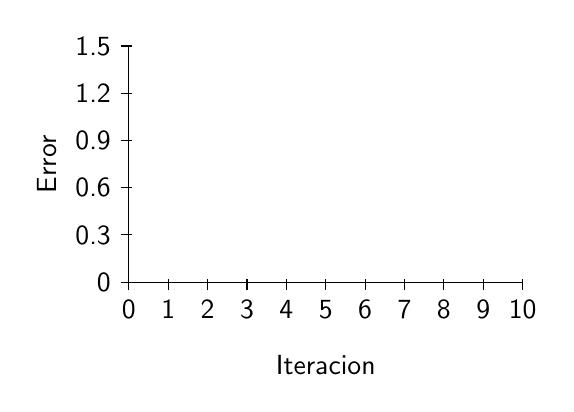
\begin{tikzpicture}[y=2cm, x=.5cm,font=\sffamily]
			%axis
			\draw (0,0) -- coordinate (x axis mid) (10,0);
			\draw (0,0) -- coordinate (y axis mid) (0,1.5);
			%ticks
			\foreach \x in {0,...,10}
			\draw (\x,1pt) -- (\x,-3pt)
			node[anchor=north] {\x};
			\foreach \y in {0,0.3,0.6,0.9,1.2,1.5}
			\draw (1pt,\y) -- (-3pt,\y) 
			node[anchor=east] {\y}; 
			%labels      
			\node[below=0.8cm] at (x axis mid) {Iteracion};
			\node[rotate=90, above=0.8cm] at (y axis mid) {Error};
			%plots
			\draw plot[mark=*, mark options={fill=white}]
			file {f2_bis.data};
			\draw plot[mark=triangle*, mark options={fill=white} ] 
			file {f2_newt.data};
		\end{tikzpicture} \\
		\hline
		\hline
		$f_4 = |x-10|$ & $f_5= - \frac{1}{32} + \frac{5x}{16} - \frac{5x^2}{4}
								+ \frac{5x^3}{2} - \frac{5x^2}{2} + x^5$ \\
		\hline
		\begin{tikzpicture}[y=1.6cm, x=.5cm,font=\sffamily]
			%axis
			\draw (0,0) -- coordinate (x axis mid) (10,0);
			\draw (0,0) -- coordinate (y axis mid) (0,1.5);
			%ticks
			\foreach \x in {0,...,10}
			\draw (\x,1pt) -- (\x,-3pt)
			node[anchor=north] {\x};
			\foreach \y in {0,0.5,1,1.5}
			\draw (1pt,\y) -- (-3pt,\y) 
			node[anchor=east] {\y}; 
			%labels      
			\node[below=0.8cm] at (x axis mid) {Iteracion};
			\node[rotate=90, above=0.8cm] at (y axis mid) {Error};
			%plots
			\draw plot[mark=*, mark options={fill=white}]
			file {f4_bis.data};
			\draw plot[mark=triangle*, mark options={fill=white} ] 
			file {f4_newt.data};
		\end{tikzpicture}
		&
		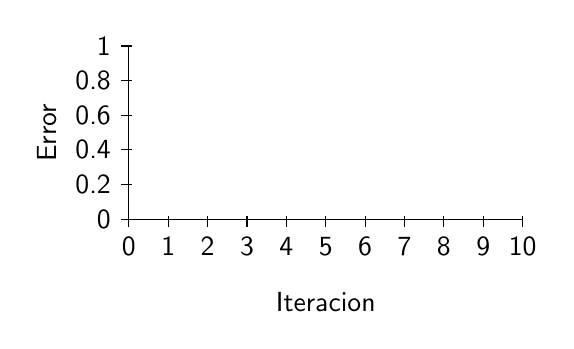
\begin{tikzpicture}[y=2.2cm, x=.5cm,font=\sffamily]
			%axis
			\draw (0,0) -- coordinate (x axis mid) (10,0);
			\draw (0,0) -- coordinate (y axis mid) (0,1);
			%ticks
			\foreach \x in {0,...,10}
			\draw (\x,1pt) -- (\x,-3pt)
			node[anchor=north] {\x};
			\foreach \y in {0,0.2,0.4,0.6,0.8,1}
			\draw (1pt,\y) -- (-3pt,\y) 
			node[anchor=east] {\y}; 
			%labels      
			\node[below=0.8cm] at (x axis mid) {Iteracion};
			\node[rotate=90, above=0.8cm] at (y axis mid) {Error};
			%plots
			\draw plot[mark=*, mark options={fill=white}]
			file {f5_bis.data};
			\draw plot[mark=triangle*, mark options={fill=white} ] 
			file {f5_newt.data};
		\end{tikzpicture} \\
		\hline
		\hline
		$f_6 =$ Bessel primer tipo & $f_7=$ Bassel segundo tipo \\
		\hline
		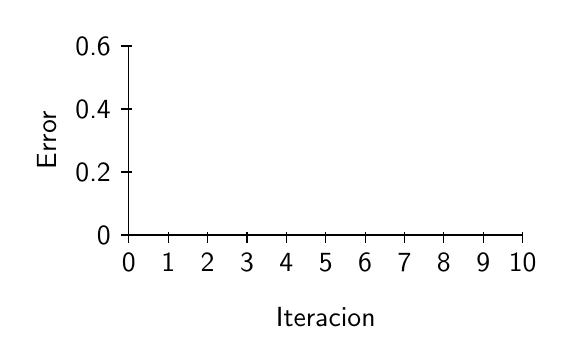
\begin{tikzpicture}[y=4cm, x=.5cm,font=\sffamily]
			%axis
			\draw (0,0) -- coordinate (x axis mid) (10,0);
			\draw (0,0) -- coordinate (y axis mid) (0,0.6);
			%ticks
			\foreach \x in {0,...,10}
			\draw (\x,1pt) -- (\x,-3pt)
			node[anchor=north] {\x};
			\foreach \y in {0,0.2,0.4,0.6}
			\draw (1pt,\y) -- (-3pt,\y) 
			node[anchor=east] {\y}; 
			%labels      
			\node[below=0.8cm] at (x axis mid) {Iteracion};
			\node[rotate=90, above=0.8cm] at (y axis mid) {Error};
			%plots
			\draw plot[mark=*, mark options={fill=white}]
			file {f6_bis.data};
			\draw plot[mark=triangle*, mark options={fill=white} ] 
			file {f6_newt.data};
		\end{tikzpicture}
		&
		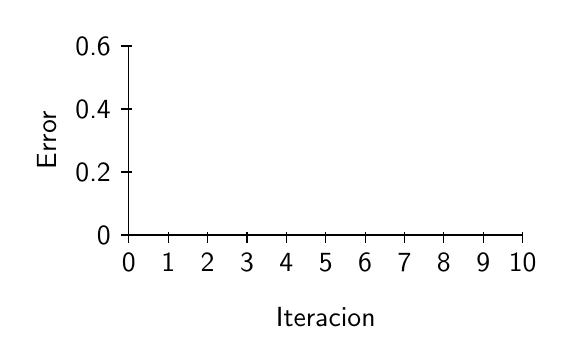
\begin{tikzpicture}[y=4cm, x=.5cm,font=\sffamily]
			%axis
			\draw (0,0) -- coordinate (x axis mid) (10,0);
			\draw (0,0) -- coordinate (y axis mid) (0,0.6);
			%ticks
			\foreach \x in {0,...,10}
			\draw (\x,1pt) -- (\x,-3pt)
			node[anchor=north] {\x};
			\foreach \y in {0,0.2,0.4,0.6}
			\draw (1pt,\y) -- (-3pt,\y) 
			node[anchor=east] {\y}; 
			%labels      
			\node[below=0.8cm] at (x axis mid) {Iteracion};
			\node[rotate=90, above=0.8cm] at (y axis mid) {Error};
			%plots
			\draw plot[mark=*, mark options={fill=white}]
			file {f7_bis.data};
			\draw plot[mark=triangle*, mark options={fill=white} ] 
			file {f7_newt.data};
		\end{tikzpicture} \\
		\hline

	\end{tabular}
\end{center}

			Notamos que en la mayoría de los casos para el método de Newton
			se llega a una solución rápidamente y con errores cercanos a cero.
			\\ Por otro lado, la bisección tiene errores que oscilan y, aunque
			terminan llegando al mismo valor, toma cerca de 30 iteraciones 
			(Dependiendo de la tolerancia definida).
			
		\item
			Tabla de comparación de iteraciones, convergencia y tiempo.
			\begin{center}
				\begin{tabular}{|r|r|r|}
					\hline
					\multicolumn{3}{|c|}{\textbf{Método de la Bisección}}\\
					\hline
					$f_i(x)$ & Tiempo & Iteraciones\\
					\hline
					$f_1(x)$ & $0.000083923339843$s	&	$27$	\\
					\hline
					$f_2(x)$ & $0.000115156173706$s	&	$29$	\\
					\hline
					$f_3(x)$ & Falló &	-	\\
					\hline
					$f_4(x)$ & $0.000063896179199$s &	$30$	\\
					\hline
					$f_5(x)$ & $0.000102043151855$s &	$29$	\\
					\hline
					$f_6(x)$ & $0.00263714790344$s &	$29$	\\
					\hline
					$f_7(x)$ & $0.00366306304932$s &	$31$	\\
					\hline
				\end{tabular}
				\qquad
				\begin{tabular}{|r|r|r|}
					\hline
					\multicolumn{3}{|c|}{\textbf{Método de Newton}}\\
					\hline
					$f_i(x)$ & Tiempo & Iteraciones \\
					\hline
					$f_1(x)$ & $0.898484945297$s &	$2$ \\
					\hline
					$f_2(x)$ & $0.00857090950012$s &	$1$ \\
					\hline
					$f_3(x)$ & Falló &	-	\\
					\hline
					$f_4(x)$ & $0.02476811409$s &	$1$	\\
					\hline
					$f_5(x)$ & $0.0450839996338$s &	$1$	\\
					\hline
					$f_6(x)$ & $0.000953912734985$s &	$6$	\\
					\hline
					$f_7(x)$ & $0.000863075256348$s &	$6$	\\
					\hline
				\end{tabular}
			\end{center}
			Cabe destacar que la tasa de convergencia de el método de la 
			bisección es lineal constante igual a $0.5$, por otro lado, para el
			método de Newton tenemos una taza de convergencia de orden superior
			, es decir, converge cada vez más rápido.
	\end{enumerate}
\section{Conclusiones}
	%Conclusiones
	Al analizar las tablas y los gráficos, queda bastante claro que el número 
	de iteraciones baja considerablemente con el método de newton, sin embargo
	los tiempos de ejecución no se condicen con esta ventaja en nuestro caso,
	como habíamos supuesto al principio. Las razones a esto último están
	asociadas al coste computacional que conlleva el manejo algebraico de las
	funciones, los cálculos de derivadas y límite, etc., funciones utilizadas
	de la librería sympy para el método de newton. Independiente de la 
	implementación, el rendimiento del método de newton se ve afectado por las
	dificultades en el computo de derivadas, las cuales no siempre son
	sencillas de resolver.\\
	Por otro lado, las funciones para el método de la bisección debieron ser
	modificadas en su mayoría, dado que varias de ellas eran estrictamente
	positivas o negativas, no así para el método de newton. Esto da una ventaja
	significativa al segundo método, dado que para hacer las modificaciones
	pertinentes, se requiere de cierto conocimiento en el comportamiento de las
	funciones, cosa que puede ser no trivial en algunos casos.   

\section{Referencias}
%Referencias
\begin{enumerate}
	\item
		Libro guía del curso, Numerical Analysis, 2nd Edition, Timothy Sauer,
		2006 Pearson Education.
	\item
		Función de Bessel, \url{http://en.wikipedia.org/wiki/Bessel_function}
\end{enumerate}

\newpage
\section{Anexo}
	%hack para acentos:
	\lstset{literate=
		{á}{{\'a}}1 {é}{{\'e}}1 {í}{{\'i}}1 {ó}{{\'o}}1 {ú}{{\'u}}1
		{Á}{{\'A}}1 {É}{{\'E}}1 {Í}{{\'I}}1 {Ó}{{\'O}}1 {Ú}{{\'U}}1
		{à}{{\`a}}1 {è}{{\'e}}1 {ì}{{\`i}}1 {ò}{{\`o}}1 {ù}{{\`u}}1
		{À}{{\`A}}1 {È}{{\'E}}1 {Ì}{{\`I}}1 {Ò}{{\`O}}1 {Ù}{{\`U}}1
		{ä}{{\"a}}1 {ë}{{\"e}}1 {ï}{{\"i}}1 {ö}{{\"o}}1 {ü}{{\"u}}1
		{Ä}{{\"A}}1 {Ë}{{\"E}}1 {Ï}{{\"I}}1 {Ö}{{\"O}}1 {Ü}{{\"U}}1
		{â}{{\^a}}1 {ê}{{\^e}}1 {î}{{\^i}}1 {ô}{{\^o}}1 {û}{{\^u}}1
		{Â}{{\^A}}1 {Ê}{{\^E}}1 {Î}{{\^I}}1 {Ô}{{\^O}}1 {Û}{{\^U}}1
		{œ}{{\oe}}1 {Œ}{{\OE}}1 {æ}{{\ae}}1 {Æ}{{\AE}}1 {ß}{{\ss}}1
		{ç}{{\c c}}1 {Ç}{{\c C}}1 {ø}{{\o}}1 {å}{{\r a}}1 {Å}{{\r A}}1
		{€}{{\EUR}}1 {£}{{\pounds}}1
	}


%Anexo con código utilizado
	\lstinputlisting[language=Python,
				 frame=single,
				 showstringspaces=false,
				 commentstyle=\color{gris},
				 title=\lstname,
			 	 tabsize=4]{../Codigos/Laboratorio2.py}

\vfill\hfill HV/AS/\LaTeXe
\end{document}
